%%
%% This is file `sample-manuscript.tex',
%% generated with the docstrip utility.
%%
%% The original source files were:
%%
%% samples.dtx  (with options: `manuscript')
%% 
%% IMPORTANT NOTICE:
%% 
%% For the copyright see the source file.
%% 
%% Any modified versions of this file must be renamed
%% with new filenames distinct from sample-manuscript.tex.
%% 
%% For distribution of the original source see the terms
%% for copying and modification in the file samples.dtx.
%% 
%% This generated file may be distributed as long as the
%% original source files, as listed above, are part of the
%% same distribution. (The sources need not necessarily be
%% in the same archive or directory.)
%%
%% The first command in your LaTeX source must be the \documentclass command.
%%%% Small single column format, used for CIE, CSUR, DTRAP, JACM, JDIQ, JEA, JERIC, JETC, PACMCGIT, TAAS, TACCESS, TACO, TALG, TALLIP (formerly TALIP), TCPS, TDSCI, TEAC, TECS, TELO, THRI, TIIS, TIOT, TISSEC, TIST, TKDD, TMIS, TOCE, TOCHI, TOCL, TOCS, TOCT, TODAES, TODS, TOIS, TOIT, TOMACS, TOMM (formerly TOMCCAP), TOMPECS, TOMS, TOPC, TOPLAS, TOPS, TOS, TOSEM, TOSN, TQC, TRETS, TSAS, TSC, TSLP, TWEB.
% \documentclass[acmsmall]{acmart}

%%%% Large single column format, used for IMWUT, JOCCH, PACMPL, POMACS, TAP, PACMHCI
% \documentclass[acmlarge,screen]{acmart}

%%%% Large double column format, used for TOG
% \documentclass[acmtog, authorversion]{acmart}

%%%% Generic manuscript mode, required for submission
%%%% and peer review
\documentclass[manuscript,screen]{acmart}
\usepackage{subfig}

\newcommand{\todo}[1]{{\color{red} TODO: #1}}   

%%
%% \BibTeX command to typeset BibTeX logo in the docs
\AtBeginDocument{%
  \providecommand\BibTeX{{%
    \normalfont B\kern-0.5em{\scshape i\kern-0.25em b}\kern-0.8em\TeX}}}

%% Rights management information.  This information is sent to you
%% when you complete the rights form.  These commands have SAMPLE
%% values in them; it is your responsibility as an author to replace
%% the commands and values with those provided to you when you
%% complete the rights form.
\setcopyright{acmcopyright}
\copyrightyear{2021}
\acmYear{2021}
\acmDOI{10.1145/1122445.1122456}



%% These commands are for a PROCEEDINGS abstract or paper.
\acmConference[C\&C 2021]{C\&C 2021: ACM SIGCHI Conference on Creativity and Cognition}{June 2021}{Venice, Italy}
\acmPrice{15.00}
\acmISBN{978-1-4503-XXXX-X/18/06}

%%
%% Submission ID.
%% Use this when submitting an article to a sponsored event. You'll
%% receive a unique submission ID from the organizers
%% of the event, and this ID should be used as the parameter to this command.
%%\acmSubmissionID{123-A56-BU3}

%%
%% The majority of ACM publications use numbered citations and
%% references.  The command \citestyle{authoryear} switches to the
%% "author year" style.
%%
%% If you are preparing content for an event
%% sponsored by ACM SIGGRAPH, you must use the "author year" style of
%% citations and references.
%% Uncommenting
%% the next command will enable that style.
%%\citestyle{acmauthoryear}

%%
%% end of the preamble, start of the body of the document source.
\begin{document}

%%
%% The "title" command has an optional parameter,
%% allowing the author to define a "short title" to be used in page headers.
\title{Sonifying Invisible Computer Processes}

%%
%% The "author" command and its associated commands are used to define
%% the authors and their affiliations.
%% Of note is the shared affiliation of the first two authors, and the
%% "authornote" and "authornotemark" commands
%% used to denote shared contribution to the research.

% THE FOLLOWING AUTHO LINES ARE COMMENTED FOR ANONYMIZING THE PAPER

%\author{Roberto Bresin}
%\authornote{All authors contributed equally to this research.}
%\email{roberto@kth.se}
%\orcid{0000-0002-3086-0322}
%\author{Benoit Baudry}
%\authornotemark[1]
%\email{baudry@kth.se}
%\author{Thomas Durieux}
%\authornotemark[1]
%\email{tdurieux@kth.se}
%\author{Erik Natanael Gustafsson}
%\authornotemark[1]
%\email{bengusta@kth.se}
%\author{Claudio Panariello}
%\authornotemark[1]
%\email{claudiop@kth.se}
%\author{Sandra Pauletto}
%\authornotemark[1]
%\email{pauletto@kth.se}\affiliation{%
%  \institution{KTH Royal Institute of Technology}
%  \city{Stockholm}
%  \country{Sweden}
%  \postcode{100 44}}

%\author{Henrik Frisk}
%\affiliation{%
%  \institution{KMH Royal College of Music}
%  \streetaddress{Box 27711}
%  \city{Stockholm}
%  \country{Sweden}
%  \postcode{115 91}  }
%\email{henrik.frisk@kmh.se}

%\author{Erik Gandini}
%\affiliation{%
%  \institution{SKH Stockholm University of the Arts}
%  \streetaddress{Box 27711}
%  \city{Stockholm}
%  \country{Sweden}
%  \postcode{115 91}  }
%\email{erik.gandini@uniarts.se}


\newcommand{\Pellow}{INSTALLATION }
\newcommand{\Gandini}{FILM DIRECTOR }


%%
%% By default, the full list of authors will be used in the page
%% headers. Often, this list is too long, and will overlap
%% other information printed in the page headers. This command allows
%% the author to define a more concise list
%% of authors' names for this purpose.

% THE FOLLOWING LINE IS COMMENTED FOR ANONYMIZING THE PAPER
%\renewcommand{\shortauthors}{Bresin and Baudry, et al.}

%%
%% The abstract is a short summary of the work to be presented in the
%% article.
\begin{abstract}
  Software fuels the digital transformation of all sectors in our society. It plays a critical role in all aspects of our lives, from health care to energy distribution, education, entertainment and governmental services. Yet, citizens hardly realize the complexity, the power and the impact of software because it is, by its nature, intangible and invisible. In this work we report on two experiments that aim at letting citizens make sense of software present in their everyday lives, through sound. These are (1) the hidden information exchanged in the communication between the internet browser and many different pages and companies around the world, and (2) the invisible complexity of the processes involved in the shut-down of a computer. 
We used sonification to transform information embedded in software through the sound domain. These two experiments share a ``double character''. They are artistic realizations (one art installation and one sonic representation of information to be used in a documentary project) that develop specific aesthetic choices, and they are also concrete resources with a clear pedagogical purpose.
\end{abstract}

 

%%
%% The code below is generated by the tool at http://dl.acm.org/ccs.cfm.
%% Please copy and paste the code instead of the example below.
%%
\begin{CCSXML}
<ccs2012>
 <concept>
  <concept_id>10010520.10010553.10010562</concept_id>
  <concept_desc>Computer systems organization~Embedded systems</concept_desc>
  <concept_significance>500</concept_significance>
 </concept>
 <concept>
  <concept_id>10010520.10010575.10010755</concept_id>
  <concept_desc>Computer systems organization~Redundancy</concept_desc>
  <concept_significance>300</concept_significance>
 </concept>
 <concept>
  <concept_id>10010520.10010553.10010554</concept_id>
  <concept_desc>Computer systems organization~Robotics</concept_desc>
  <concept_significance>100</concept_significance>
 </concept>
 <concept>
  <concept_id>10003033.10003083.10003095</concept_id>
  <concept_desc>Networks~Network reliability</concept_desc>
  <concept_significance>100</concept_significance>
 </concept>
</ccs2012>
\end{CCSXML}

\ccsdesc[500]{Computer systems organization~Embedded systems}
\ccsdesc[300]{Computer systems organization~Redundancy}
\ccsdesc{Computer systems organization~Robotics}
\ccsdesc[100]{Networks~Network reliability}

%%
%% Keywords. The author(s) should pick words that accurately describe
%% the work being presented. Separate the keywords with commas.
\keywords{software processes, data representation, sonification, sound design, sound and music computing}


\begin{teaserfigure}
    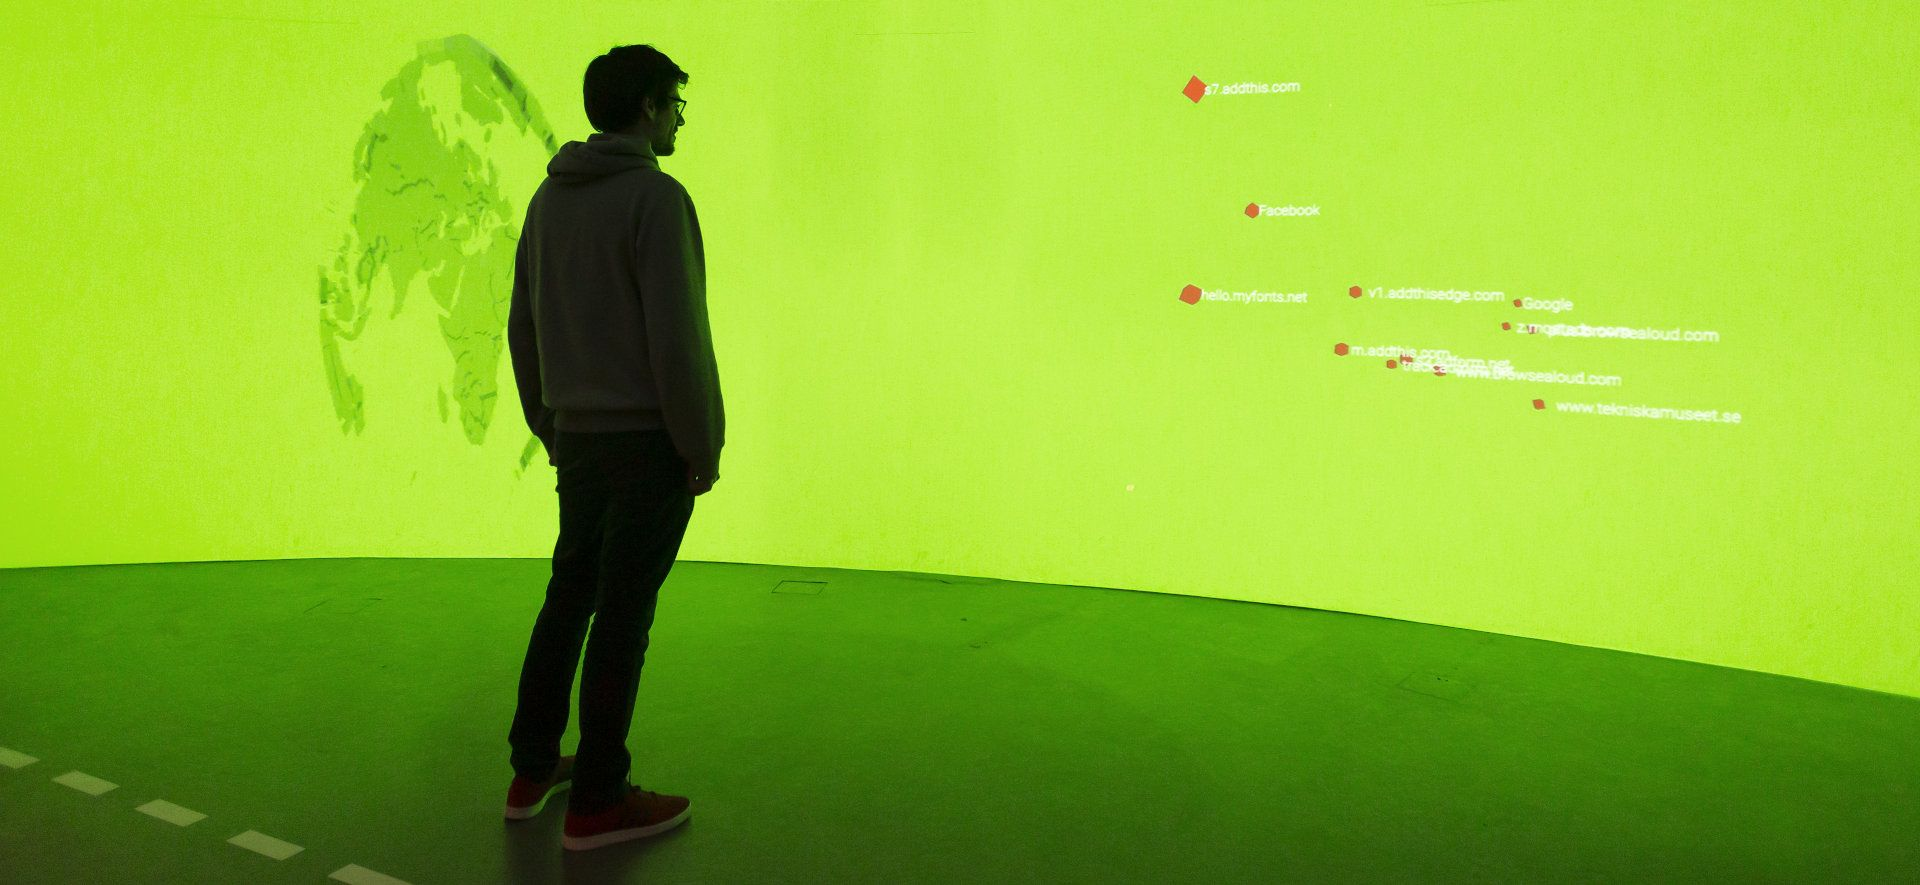
\includegraphics[width=\textwidth]{images/pellow-tekniska-anne-gerden.jpg}
    \caption{\Pellow, a browser art installation that lets users explore the web anew, through sonification and visualisation. Exhibited at TECHNOLOGY MUSEUM 
    %Tekniska Museet, Stockholm, Sweden, October 2020.
    }
    \Description{\Pellow, a browser art installation that through sonification and visualisation lets users explore the web anew.}
    \label{fig:pellow_large}
 \end{teaserfigure}
 
 
%%
%% This command processes the author and affiliation and title
%% information and builds the first part of the formatted document.
\maketitle


  
\section{Introduction}

``Software is eating the world!'' \cite{andreessen2011software}. Software is the core medium that fuels radical digital transformations in all sectors of our societies, from health and energy to business, labour and culture  \cite{manovich2013software}. Yet, software is an invisible and intangible set of processes that run millions of operations per second, on top of world-wide networks. Consequently it is very difficult to make sense of software and its effects on society. Meanwhile, there is a growing curiosity and concern among citizens who use digital technology about the nature, the role and the influence of software  \cite{solove2004digital}. 
Societal questions span privacy and surveillance \cite{hintz2017digital}, freedom of choice and filter bubbles \cite{nguyen2014exploring}, social exclusion \cite{Hargittai08} or environmental concerns. Furthermore, the underlying technologies may have hidden biases that affect the information the user is provided with \cite{snow2018}.


To give ``voice'' to and to some extent reveal this otherwise invisible and silent software medium, we investigate the use of sound and its intrinsic property of involving our brain and body in its experience \cite{kohler2002hearing}. Listening  activates our premotor cortex for making sense of sound through both simulated, imagined and enacted movements \cite{caramiaux2014role}. Sound allows for both an intimate (headphones) and collective (sound installations) experience of the software activity \cite{Eckel2016zeitraum}. 

This work introduces two experiments that aim at revealing an aspect of software through sound. The first experiment focuses on a software component that is essential to our online presence: a web browser and its interactions with the world-wide web. The second experiment explores a usually unnoticed, yet fundamental, software phenomenon: the shutdown of a digital device. 
%\todo{elaborate on the content of the paper}

\section{Background}
\subsection{Representation of complexity of software processes}

The complexity of software emerges in various forms. Some notable forms of software complexity are related to: speed,  software operates at very high frequency; mass, user actions are split into a very large amount of interconnected operations; width, most software applications operate across multiple devices located in different locations; autonomy, a large number of software operations are performed autonomously, with no explicit human trigger; intangibility, the most challenging property of software is that it is invisible and intangible. Works that aim at revealing this polymorphic complexity need to address the following key questions: what part of software do we focus on? How can we observe it? What medium do we use to represent and make sense of it? In an engineering context, the answer to the first question is usually  guided by the aspects that affect the performance of the application, while in the context of software studies, the choice is guided by societal impacts of software. The second question requires some advanced software technology, whatever we wish to observe, and is usually referred as observability \cite{Sridharan18}. Mathematics is commonly used to answer the third question in a computer science context, whereas media that call more directly to our senses, such as images or sound, are usually used in software studies.

\subsection{Sonification: Portraying data with sound}
%Roberto and Claudio and Henrik
The ability to make sense of sounds is generally taken for granted \cite{mcadams1993}. Humans can, with some experience, distinguish and make sense of a large set of different sounds. Examples include everything from distinguishing different musical instruments in an orchestra to recognizing footsteps of someone who is familiar \cite{mcadams1993}. 

Sound is the best modality for, among other things, representing and communicating the invisible, and for raising awareness -- as in alarm sounds or in movies. Imagine a scene in which we hear, but not see, a door that is opening and closing, and suddenly we see a new actor entering the scene. We understand, only from the sound, that the actor has just entered the room, and depending on the sound of the door, we can also have a clue about his/her intentions, mood, and material of the door \cite{houel2020perception}. Sound can make complex events, otherwise often difficult to grasp, accessible to humans. Importantly, sound is a multidimensional information carrier, and with a single sound it is possible to communicate information about many variables simultaneously. Consider for example the case of walking step sounds; from the sound of a few steps, humans are able to recognize gender, age, weight, size, material of shoes and floor, mood and pace of a person walking \cite{visell2009sound,giordano2014production}. Even the direction the person is walking in may be discerned.

Sonification is a rather young discipline, translating data into mostly non-speech sound in a systematic and reproducible way. The main community of sonification research is formed around the International Conference on Auditory Display (ICAD) and its proceedings\footnote{\url{https://smartech.gatech.edu/handle/1853/49750}}. However, sonification is also part of many sound artist's practicies where a more varied range of approaches may be found. In artistic sonification getting the perceiver to focus their attention to details of ordinary life such as background noise, chattering, interference is an important aspect of this practice \cite{tittel2009sound}. \textit{Data Sonification}, on the other hand, can be regarded as an offline data presentation technique by means of an audio signal that has a strict and well defined mapping between data an sound.

Acoustic variables such as sound frequency, sound pressure level, envelope, timbre, rhythm, can portray features of arbitrary data \cite{dubus2013systematic}. The state-of-the-art in data sonification is that sonifications are almost always ``individual unique designs'', that is, that there is no established and accepted practices how to turn stream-based data into sound for arbitrary data.  

\textit{Interactive Sonification}\footnote{ The state-of-the-art in Interactive Sonification is documented in the Proceedings of the Interactive Sonification workshops \url{http://interactive-sonification.org/}.} is an emerging field of research, which focuses on the interactive representation of data by means of sound, and it is therefore more suitable when real-time feedback is needed \cite{hunt2011interactive,bresin2012interactive}. This technique is particularly useful when interacting with a large amounts of data where a graphical display would be difficult to interpret due to the limited size of the display. Interactive sonification could be defined as the acoustic counterpart of interactive visualization \cite{spence2006information}. Interactive Sonification makes use of sound for exploring data in a fast and meaningful way, and it is especially suitable for data that change over time and at different hierarchical levels, such as in the execution of programming code \cite{barra2002multimodal,DebashiVickers2018}. A current trend in ISon is the recognition that data interpretation and understanding through interactive exploration is a promising target area for interactive sonification that also addresses the aesthetic value of the process.

The combined knowledge contribution from all of the above-mentioned research and artistic areas can serve as a foundation for design of auditory displays for meaningful and affective interaction and effective communication. Building on knowledge from all of these fields, high-level sound models can be designed to be used as interactive sound-based display tools, enabling expression of both meaning and emotions in general, and creating an interactive experience of high pliability for the end user \cite{lowgren2009toward}.
Unfortunately, since this is traditionally a field primarily explored by engineers, the aesthetic qualities of the generated sounds have been left out or have only been marginally considered until the recent interest in sonification from musicians and composers as an artistic practice \cite{barrass2011sonification, vickers2014sonification}. Merging the data representation aspect with an aesthetically and artistically meaningful experience for the user is an area to which we want to contribute with the studies presented in this paper.




\subsection{Software data}

Software is composed of processes that collect, process, and produce digital data. 
This data and its processing can have different forms and can be more or less visible. 


\subsubsection{Big, fast, world-wide}

Software is meant to manipulate and produce data. Every single piece of software would have no purpose and would not work without data.
The complexity, size, and interconnection of the software keeps increasing year after year. 
This is made possible by a constant increase a compute power.
The most powerful computer cluster in 2020 has been created by individuals by providing the resources of their computer to the \textit{folding@home} project. \textit{folding@home} is a distributed computing project for simulating protein dynamics. It brings together citizen scientists who volunteer to run simulations of protein dynamics on their personal computers. The projects got extremely popular during the coronavirus pandemic \cite{zimmerman2020sars}.
Together, they reach, for the first time, an exascale cluster of computers. \footnote{Exascale computer can calculate at least $10^{18}$ floating-point operations per second.} 

Only the scale of the total amount of data stored by man-kind can be compared to this massive computing power. 
The International Data Corporation, IDC, predicted that the global datasphere will grow from 33 Zettabytes in 2018 to 175 Zettabytes by 2025 \cite{rydning2018digitization}.\footnote{a Zettabytes is 1,099,511,627,776 gigabytes and would take 1.8 billion years to download with an average internet speed.}
This exponential increase can be explained by the value of data, data is precious, desired, protected, exchanged, and more importantly sold. 
Every major company is now tracking and collecting data from their clients to create some client profiles that can be sold or used to increase their margins.

The total amount of data stored by man-kind is impressive however also single software required a tremendous amount of data to execute. The Machine learning systems are part of one of those techniques that are particularly data-hungry.
% software bigger
GPT-3 \cite{brown2020language}, the largest deep learning language model, has been trained by OpenAI on 45 Terrabytes of data. It is estimated \cite{GPT3Overview} that it cost at least 4.6 million dollars to train this model. 
An additional 100,000\$ machine is required to be able to use this model.

Software data is the image of our society, getting biggest, faster, and more and more interconnected. 

\subsubsection{Two examples: World-Wide-Web and Atomic Computer operations}

The World-Wide-Web is the most iconic representation of software data. 
It is an interconnected, decentralized structure that has been originally created to share information. 
The number of websites is constantly growing, providing information, new services, and new content to any device that has an internet connection.
The complexity of webpages is increasing.
Over the last 10 years, the median size of a webpage has been increasing by more than 300\% according to HTTP Archive. \footnote{\url{https://httparchive.org/reports/page-weight?start=earliest&end=latest&view=list}}
Moreover, it is now the norm to have webpages that include resources from other platforms such as Facebook, Google, Amazon, Twitter, or Instagram. 
The goal for the website owners is to provide content to their users, such as a tweet or a picture, or to track them, e.g., Google Analytics.
The general public does not realize that when they access a website, they communicate not only with the website but also with Google, Amazon, Facebook, Twitter, and Instagram.
All those providers can, therefore, collect the data on the users even if they don't use those platforms.
This phenomenon of having more than one provide per website has an exception. 
This exception is the websites of those giants which keep for them-self the information that they can collect on their users. In Section \ref{sec:case1} we present a case study where we highlight the complexity and the interconnection of the internet activity.

Another crucial piece of technology that everybody uses every day are the operating systems.
The role of the operating system such as Windows, Mac, or Linux is to provide a set of features for the users to their computers or smartphones.
But it also provides features for developers to help them to create their software. 
It allows for example the developers to be able to write data to a drive or to use the internet without paying attention to which piece of hardware is actually used. 
The operating systems are performing an enormous amount of work when the computer is used but also when it is not.
The role and the amount of tasks that the operating system is doing is something that users are not aware of. 

In Section \ref{sec:case2} we present our second case study that illustrates this complexity of the operating system. 
We illustrate an iconic event which is the shutdown of a personal computer. When a user closes a computer its operating system increases its activity to save and remove data, orchestrate the shutdown of all the services, and preparing the machine for its next start.

\subsection{Communication of information in documentary film making}\label{sec:documentary}

As an art form and film genre, documentary film has traditionally remained within two chronological axes: the present and the past. In a current project
% THE FOLLOWING FOOTNOTE IS COMMENTED FOR ANONYMIZING THE PAPER
%\footnote{\href{https://www.uniarts.se/english/research-and-development-work/research-projects/the-future-through-the-present}{The future through the present}}
, co-author film director  \Gandini explores a documentary narrative that communicates with the future. The aim of his project is to develop a cinematic narrative that frees documentaries from the narrow-mindedness of the role as portrayer of either the contemporary or the past. Explore the possibility of grasping what is to come through projections into the future, such as the universe of imaginary ideas, hopes, hypotheses and utopias that this chronological dimension holds. This will produce new knowledge about the future narrative for documentary film.

The approach to sociology is a natural part of \Gandini's method. Sociology is described as the science that studies how people's lives are shaped by what ``is hidden'', and this has a strong similarity with the goal he has with his own films. In \Gandini’s words \textit{``Capturing the present while it is happening, grasping it 'in time', is part of my artistic vision''}. If the ambition to make sense of the present is a challenge difficult enough, the desire to do the same with the future is probably overconfident. With this research project, \Gandini wants to do just that, experiment with a documentary aesthetic that, based on a ‘what if’ attitude, examines the hypothesis of a near future where work is less and time is plenty. How will work be redefined? How will the current role of work as the center of our existence be challenged? How will the importance of professional identity change? What will happen to us when we’ll have a surplus of time?

In essence, the aim is to film the present to capture the future. The future is in documentary film  underrepresented, largely absent, a chronological dimension hitherto owned by fiction, monopolized by the sci-fi genre. With the project, \Gandini  wants to investigate the possibilities of creating a projection forward in time and do so with a traditional, authentic documentary imagery. Explore if a documentary based on material recorded in the present can create a future projection. Do that through a new documentary aesthetic for the future that is not an imitation of fiction or of the Sci-Fi genre. Instead based on documentary film's own narrative elements.

Sonification is a method for portraying and communicating what is ``hidden''. Software data are hidden to lay-persons and end users and they can made be ``visible'' by sonifying them. This sonic rendering of information can help in representing the ungraspable, make it accessible and project the listeners into future scenarios, such as that of sonic dramaturgical representation of software data.  
The notion of ‘revealing what is hidden’ is not only the common goal of the above mentioned ongoing projects. Through positioning us at the crossroad where sociology, documentary film and sound (sonification)  meet, in terms of goal rather than methods, we are creating the potential for combining different disciplines with a common aim of producing useful and necessary knowledge applicable on a broader scale. This is investigated in Case study 2 presented in Section \ref{sec:case2}.
  

\section{Case study 1: Unveiling internet activity}\label{sec:case1}
%% Erik Gustafsson + Thomas + Benoit + Henrik  

\Pellow (\textit{its real name has been anonymized for the review process}) is an audiovisual installation shown at a TECHNOLOGY MUSEUM {its real name has been anonymized for the review process}
%Tekniska museet in Stockholm
, focused towards unveiling the activity that goes on beneath the surface of the web browser. When you browse a web page, the browser commonly communicates with many different pages, machines and companies around the world. \Pellow lets you see and hear this communication, intended to fetch the content that the user requested. As they press a link in the installation interface the user gets to observe where the content is fetched from and how many organizations and machines are solicited to deliver the web page requested. A sonification of these sometimes intense software exchanges complements the visual representation in order to allow for a full experience of the complexity of a web browser and its communications.

The data is collected using a browser add-on installed on a computer with a touch screen (see Fig.~\ref{fig:pellow_vis}b). As mentioned above the visitor interacts with the installation by browsing the web through the touch screen installed in front of a projection of the visuals. Through the add-on, we have full access to each request the browser makes for any content on the Internet, as well as the content type (e.g. images, scripts, fonts, css) of each request.

%% \subsubsection{Sonification}

Sonification of the web browser activity happens on two different levels simultaneously: direct sonification, and sonification of accumulated data. Requests are directly sonified with a short noise impulse to give a sense of the frequency of requests being sent and received. If a request is \textit{to} or \textit{from} one of several predefined large Internet actors (among them Amazon, Facebook, Google and Microsoft) a recording of the name of that company being whispered is heard, although sometimes slightly disguised. This lets the listener hear how prevalent these services are even for webpages that have seemingly nothing to do with them. As the names are whispered they contribute to the already quite complex soundfield portrayed by the installation. The recorded voice is originally adult female, but the fact that it is whispered and pitch shifted somewhat obscures the perceived gender and age of the voice.

Web page activity is also sonified in terms of the currently browsed webpage or web session. A background chord is played whenever there is Internet activity related to the browser. Its harmonic complexity, timbral brightness, temporal fragmentation, and spatial width depend on the data accumulated for that webpage: the number of different IP addresses that have been contacted, the number of requests that have been made, what ratio of these requests are to the original URL accessed by the user as opposed to other URLs, how many scripts are run on the page and how many requests have been made for additional data from such scripts (so called AJAX requests). Each of these metrics control one or several sound synthesis parameters through the application of a suitable transfer function between the original curve of the values for a specific metric and a curve to make that metric audible in a specific sound synthesis parameter. For example, the timbral brightness parameter depends on the ratio of requests coming from the URL in the address bar and maps that data onto the relative mix of two synthesis waveforms, one being a pink noise generator through a resonant filter, the other being a detuned pulse width generator with medium width. The harmonic content is chosen from a list of chords with increasing dissonance, from pure fifths to microtonal chromatic dissonances. Additionally, every new request made increases the intensity of a percussive sound in a 4 bar grid, adding rhythmic patterns.

Combined, the listener is able to hear both the immediate web requests coming through and the overall activity of the entire web page. Musical considerations and judgements have been made in the sonification that go beyond mapping data to sound, which points to the aforementioned ambition to also consider the aesthetic aspect. Each new web page request results in a new mini-composition that is similar, yet different, to the prior events. Each such mini-composition is structured as a piece of music, but one where many of the time based and harmonic parameters are structured from the data based on a set of possibilities. With rudimentary knowledge of how music is structured it is possible to understand quite many details about the data streams that are otherwise hidden from the users. All sound synthesis is done in real time in SuperCollider\footnote{\url{https://supercollider.github.io/}}.

Sound examples are available in THE MP4 VIDEO ATTACHED TO THIS SUBMISSION.  
% THE FOLLOWING LINE IS COMMENTED FOR ANONYMIZING THE PAPER
% at \url{https://doi.org/10.5281/zenodo.4541186}\cite{pellow_sound_examples}

%%\subsubsection{Visualisation}

The \Pellow visualisations are projected onto a curved wall in the installation space \textit{Visionslabbet}. They feature two aspects of the data visualised side by side: the names or URLs of the services being communicated with and the location of the servers being communicated with (see Fig.~\ref{fig:pellow_vis}c). These visualisations are important, not only for the information about the data that they communicate to the viewers, but also to connect the web page that the visitors have browsed to the sounds being played in the room. The visuals include clues such as recognisable strings of text and the timing of new shapes appearing that let visitors know that the entire installation depends on their interaction with the web browser on the touch screen. In this sense the visuals complement the sonification and offers the user a way in to the installation and encourages interaction.

\begin{figure*}[!t]
\centering
\subfloat[][\label{fig:data_write}]
{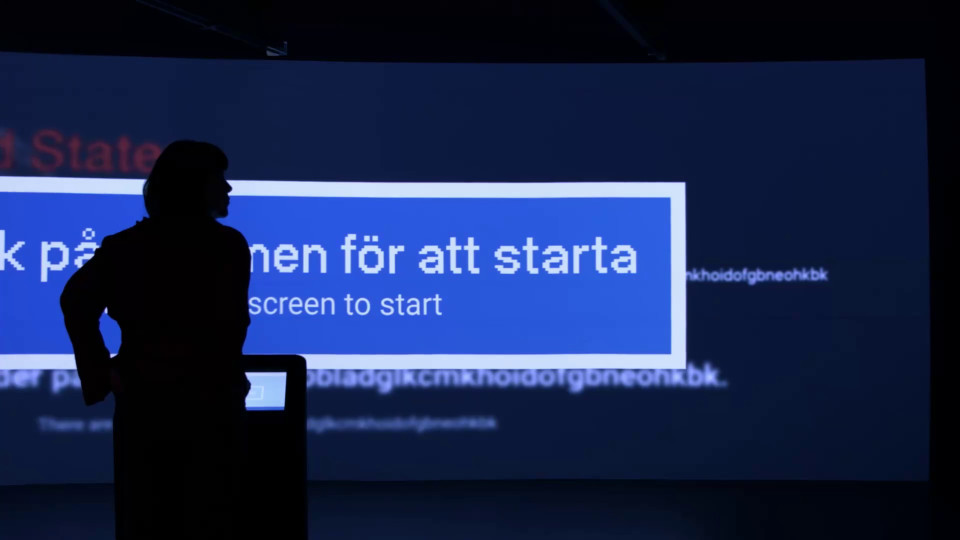
\includegraphics[scale=0.15]{images/pellow1.jpg}}
\subfloat[][\label{fig:data_exit}]
{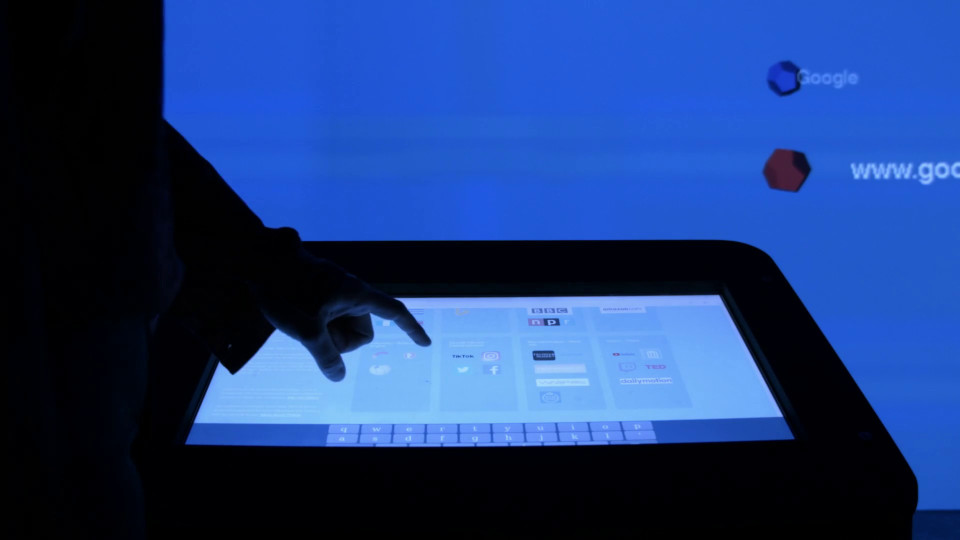
\includegraphics[scale=0.15]{images/pellow2.jpg}}
\subfloat[][\label{fig:data_kill}]
{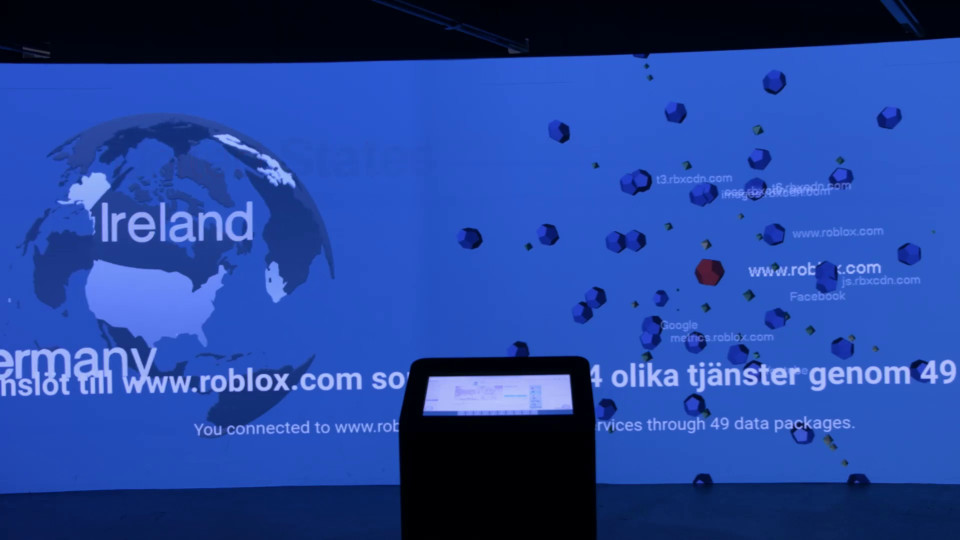
\includegraphics[scale=0.15]{images/pellow3.jpg}} 
\caption{\Pellow at TECHNOLOGY MUSEUM. a) start screen, b) touch screen interface, c) visualisation of visiting the website roblox.com.}
\label{fig:pellow_vis}
\end{figure*}
%% TODO: Image of the installation

%%\subsection{Evaluation}

The installation was shaped by the space and the audience it was intended for. A large curved projection wall that dominated the room let us put two visualisations side by side (see Fig.~\ref{fig:pellow_large} and Fig.~\ref{fig:pellow_vis}a). The target audience, consisting largely of children, could not be assumed to have their own digital devices with which to connect to the installation, which is why we opted for a touch screen interface, limiting the installation to one person at a time. This meant the personal connection between your own device and the data it produces was not there, but on the other hand we were able to have a more comprehensive data capture solution on the web browser on the touch screen instead. There is much to be said about the advantages of allowing users to interact with their own devices compared to using a stationary computer, but in this case it appeared to be the best option to use an installed, fixed computer.

The installation was approached by and engaged with by the visitors of TECHNOLOGY MUSEUM
%Tekniska museet 
who were mostly children around the age of 10-14 and their families. Many of the visitors were amazed by the amount of activity that web browsing created. Some visitors were alarmed by the prevalence of the tech giants on the Internet and on pages that had seemingly nothing to do with them. Other visitors had a playful approach of the installation, browsing web sites and looking to trigger large amounts of sound and colors. Common for most visitors was realizing the complexity of actions that they all considered trivial and mundane. The audiovisual installation let all visitors get a glimpse into an apparent contradiction between the sense of extreme familiarity with web browsing and the realization of the extreme  complexity of software in the browser. 

\Pellow only scratched the surface of what could be possible with the data we had access to. From a pedagogical point of view more could be done, and the idea of rendering visible the activities under the hood of the computer surfing the web is important. Only considering the way \Pellow shows how centralized data is, concentrated in North America and a few countries in Europe, is an extremely important insight, not only for children, and not least in relation to the discussion on bias in software models mentioned above.

\section{Case study 2: Sonification of a personal computer shutdown}\label{sec:case2}

In a scene in the documentary project presented above, several personal computers in an open space office are automatically shutdown. This is done in an attempt from public authorities in a specific Asian country to make employees stop working at a specific time in the late afternoon so that they leave their office and go home to spend more time with their families and/or in leisure activities. 

The sonification of a personal computer shutdown starts from a very large amount data: a collection of all the processes going on when a computer receives the instruction to shutdown. Since the time distance between two collected events was of $10^{-8}$s in general, the data were grouped into larger windows of time (0.1 s) to make it more manageable from an audio point of view.
The sound design process, which is still ongoing, so far went through different phases. At the beginning, a mere translation of the events into the audio domain was done by means of sine waves with a percussive envelope. This was a fairly simple sonification which aim was to get acquainted with the data and to look for possible musical pattern to investigate further.


In the following sound design stages, ideas about how we would have liked the final result to sound started to be part of the process. This does not mean that the data were changed in order to achieve a particular sound output, rather it affected the design of the synthetic sounds then used for the sonification.
We decided to look at the sonic characteristics of the Glitch (and post-Glitch) scene. Conceptually, Glitch music is a genre of electronic music that started emerging in the  early 1990s making a deliberate use of glitch-based sound materials, distortions, aliasing, quantization noise and all the ``failures'' of digital technologies~\cite{cascone2000aesthetics}. With this in mind, it seemed interesting to try and use this aesthetic to sonify the PC-shutdown using a dramaturgy of the ``PC death''. This approach was inspired also by the data itself, since they contain all the process recorded when a shutdown is launched and categorized as “write”, “ext” and “kill” events (see Fig.~\ref{fig:data_events} for three plots of these events).

\begin{figure*}[!t]
\centering
\subfloat[][\label{fig:data_write}]
{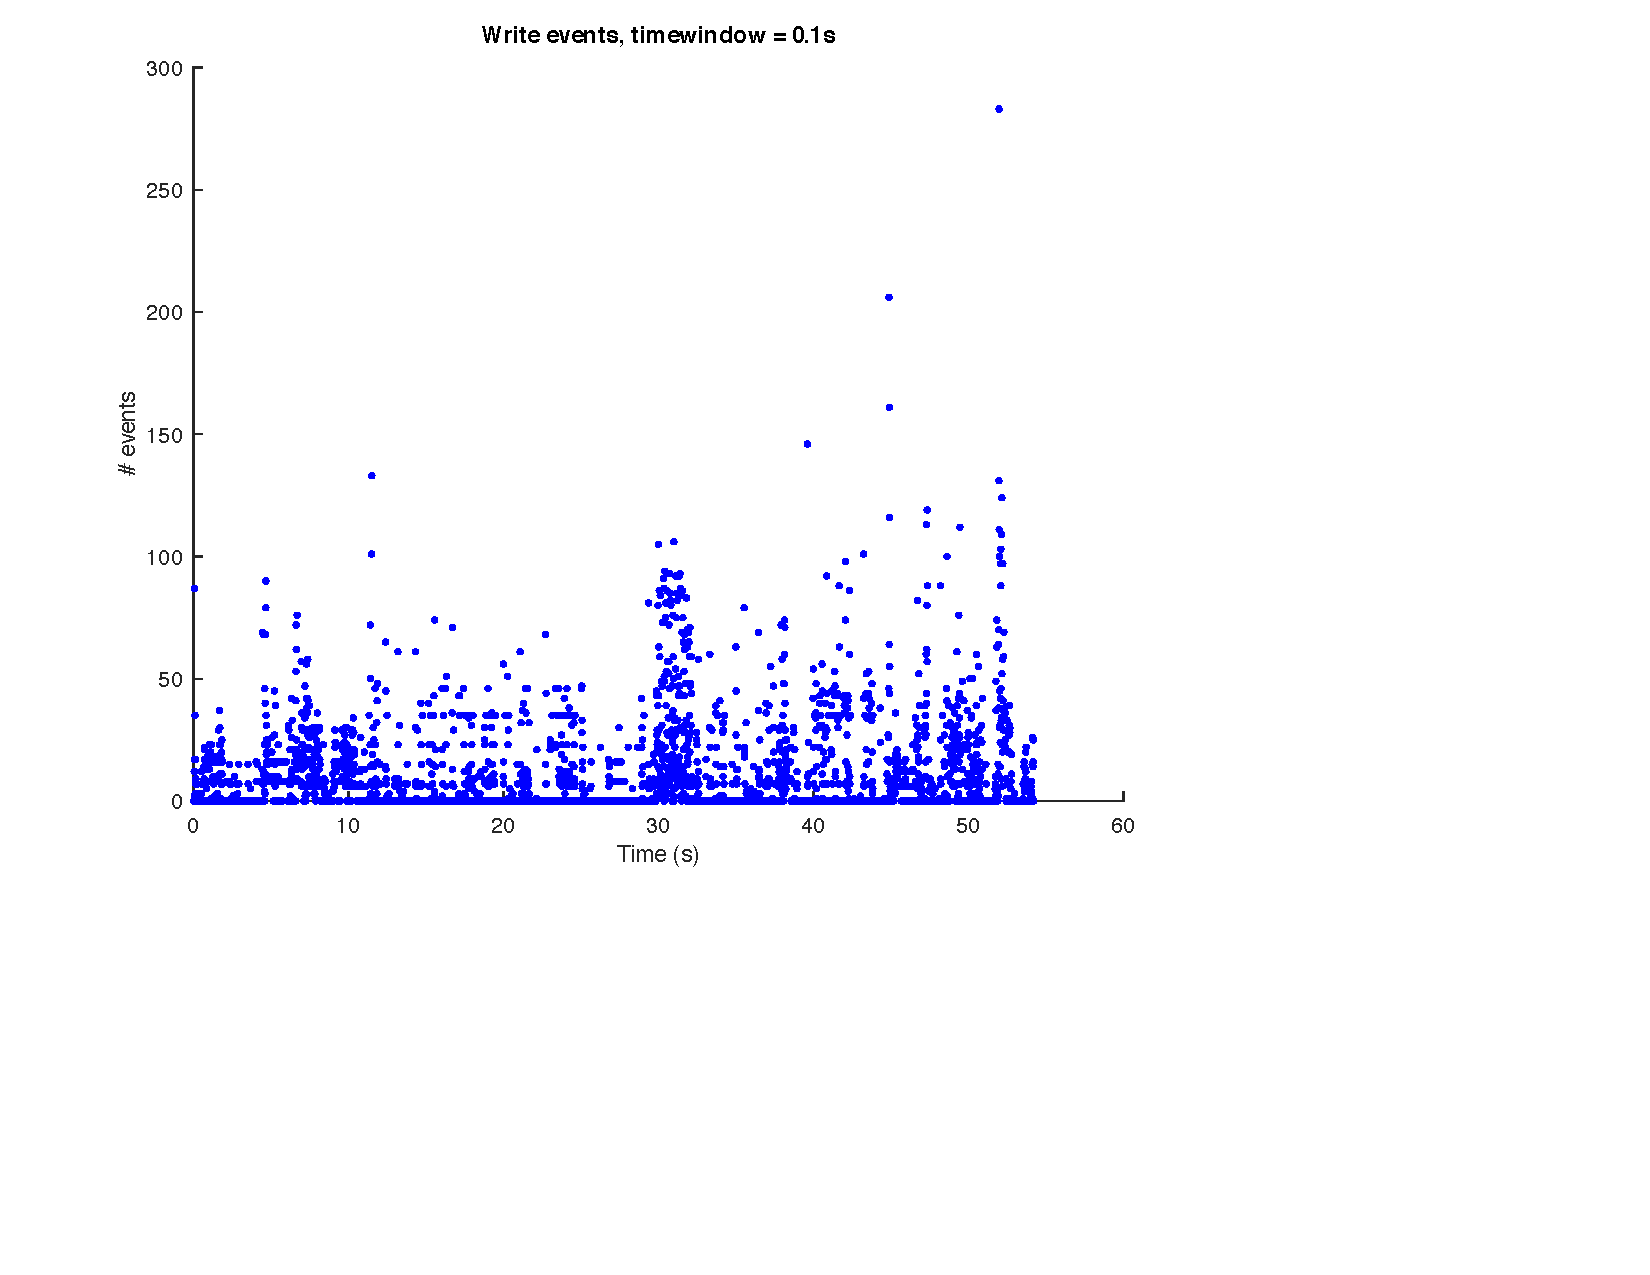
\includegraphics[scale=0.3]{images/data_write.pdf}}
\subfloat[][\label{fig:data_exit}]
{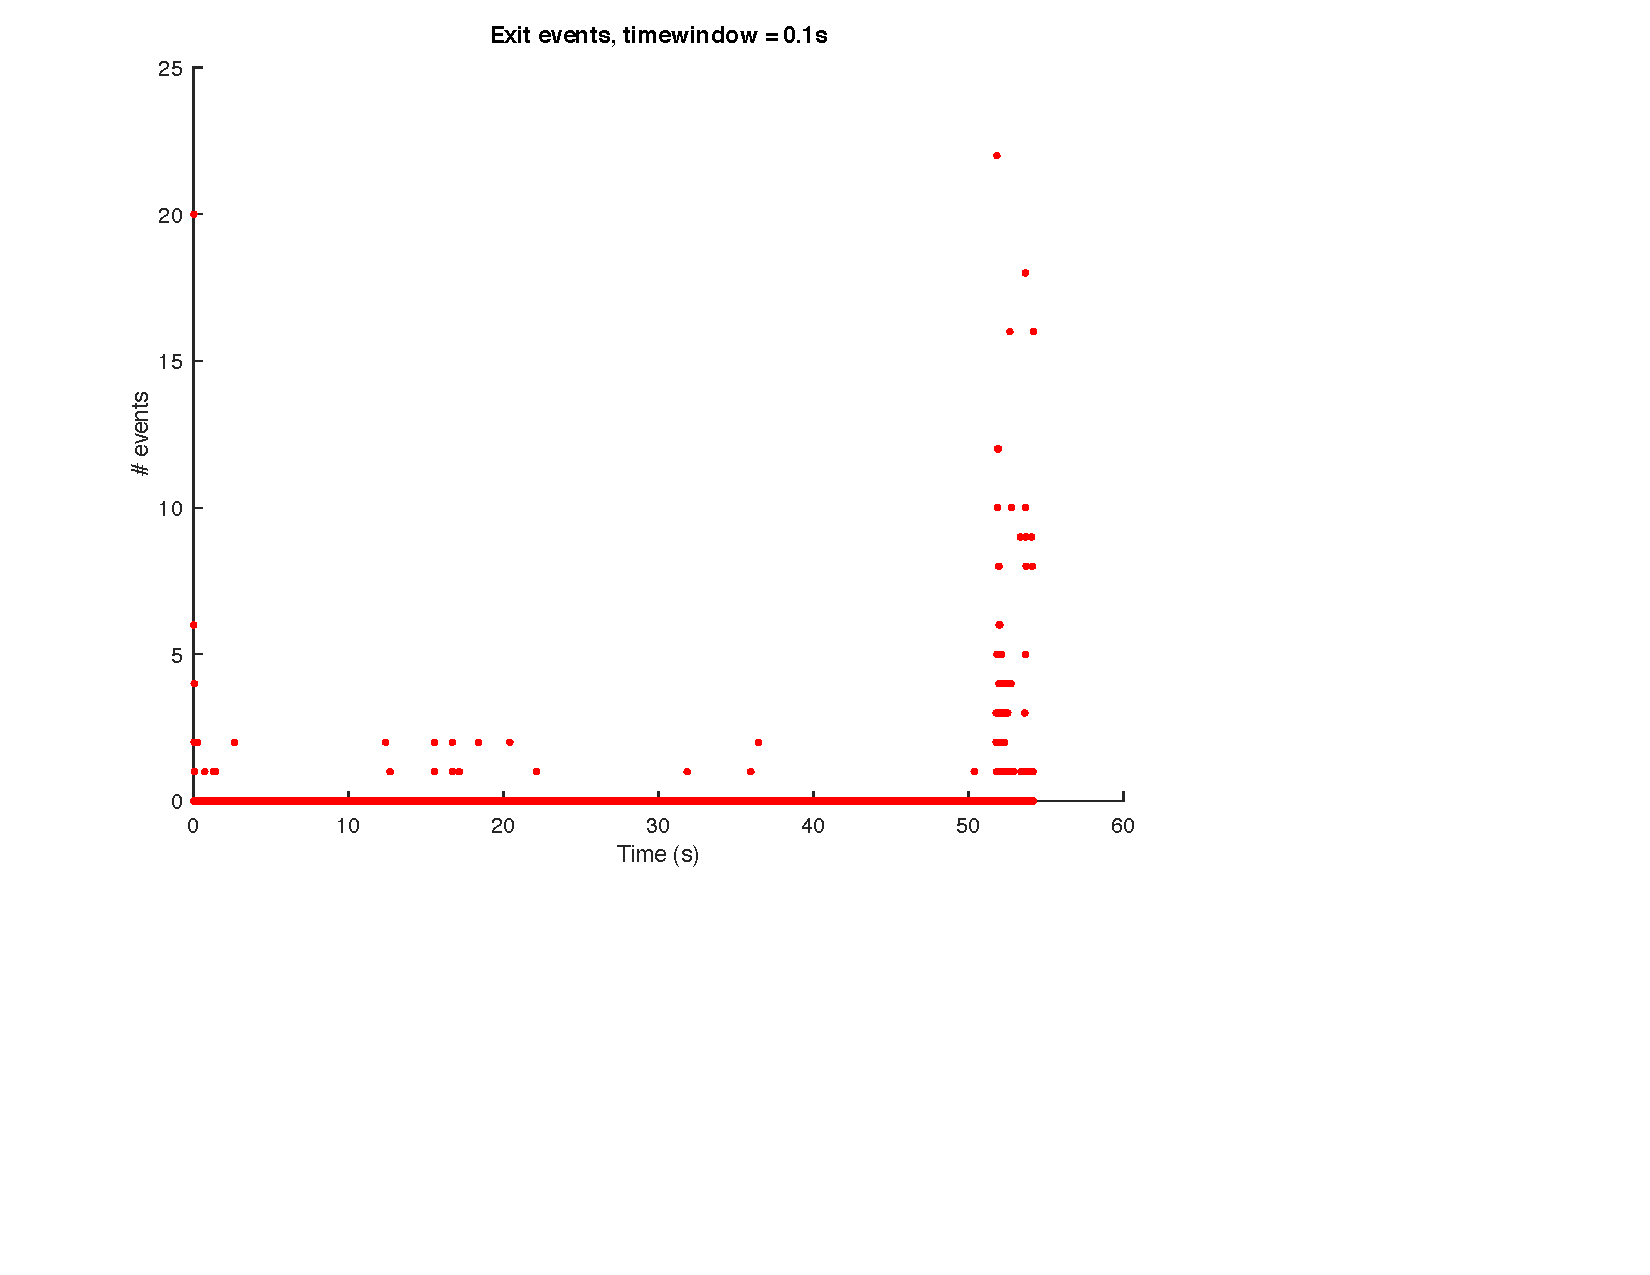
\includegraphics[scale=0.3]{images/data_exit.pdf}}
\subfloat[][\label{fig:data_kill}]
{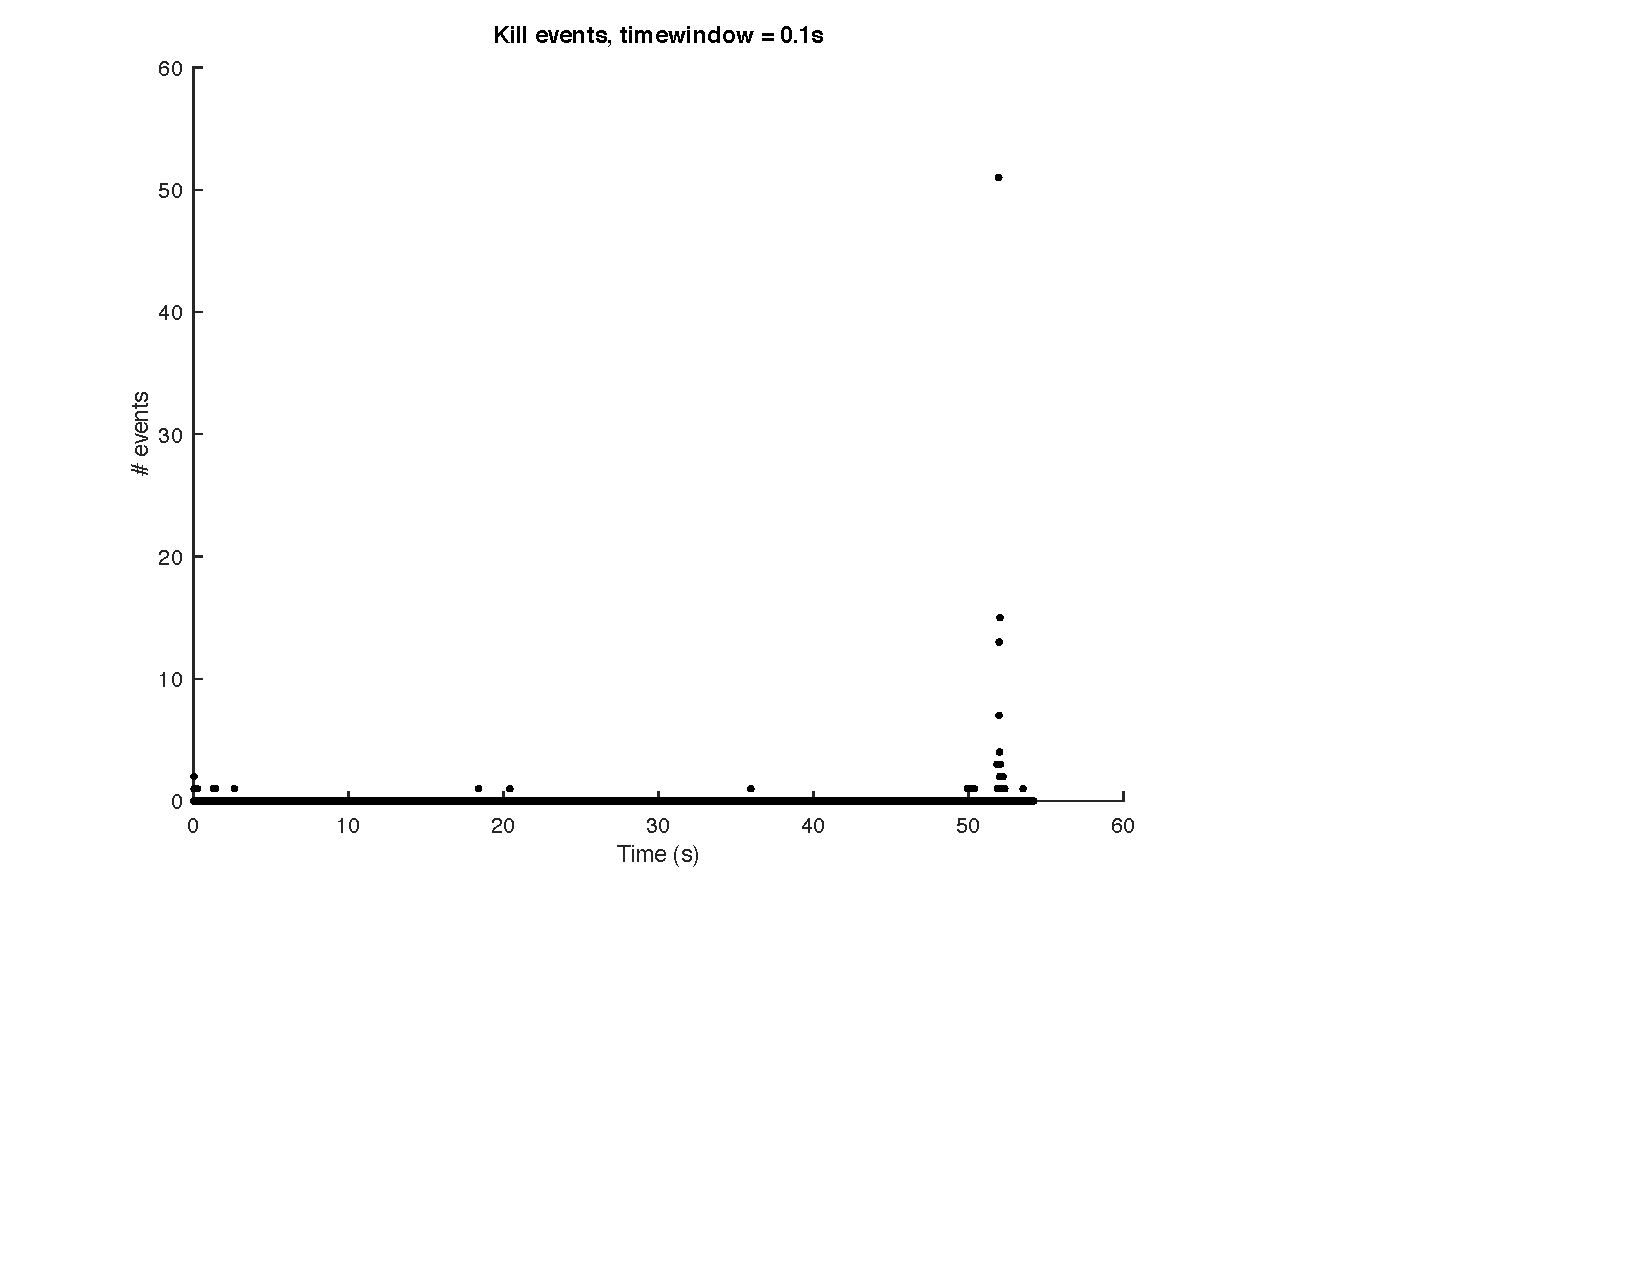
\includegraphics[scale=0.3]{images/data_kill.pdf}} 
\caption{Amount of "write" events, "exit" events and "kill" events per window of time (0.1s).}
\label{fig:data_events}
\end{figure*}



In the latest stage of sound design, the one presented here, the sonification is a result of four interconnected sound layers. The first three are the “write”, “ext” and “kill” events collected in the shutdown, and the fourth one is following the density of overall events over time.
The Sonification was realized in SuperCollider.

The sonification of the write events makes use of a granulated harmonic sum of sinusoids and of the UGen Gendy1, a dynamic stochastic generator conceived by Xenakis \cite{xenakis1992formalized} and coded in SuperCollider by Nick Collins \cite{collins2011implementing}.  The fundamental frequency of the sinusoids, the size of the grains and the overall sound level are all mapped (in different ways) to the number of write events per window of time. Write events are seen here as positive events, since they are saving data on server for future use, and we therefore sonify them using high frequency sounds which are characteristic for the communication of positive emotions such as happiness~\cite{bresin2011emotion}.
The result is a high pitched glitch texture, almost constant for the entire shutdown process (due to the continuous writing processes) and with an increasing of activity towards the end, when the majority of writing events accumulate. 

The sonification of kill events is created by means of a sinewave with a parametric envelope with a sharp attack and variable release time. Since the distribution of the kill events is quite sparse, we have decided to map the number of these events per window of time not only to sound level and fundamental frequency, but also to the actual number of sounds overlapping. In this case, the fundamental frequency has been chosen in the low range (oscillating around 40 Hz), obeying to basic sound perception rules that associates low frequencies to sad or scary emotions~\cite{bresin2011emotion}.
The result is an erratic and menacing layer of low hits, interesting from a mere musical point of view since it involuntarily increases the overall drama.

The sonification of exit events is created with a bandpass filter applied to pink noise multiplied by an impulse with decay. The aim was to create sharp explosive glitch sounds.
Also here, the number of exit events per window of time has been mapped to filter's central frequency and to impulse frequency. The frequency range in this case is in the middle-high (500-1000 Hz). Since exit and kill events are connected, the flow of exit glitches follows the low layer of the kill ones, creating a sort of musical counterpoint.

Finally, the fourth layer is drone created by the granulation of an input sound made up of 6 summed harmonic sinusoids. A curve obtained drawing a contour of the density of events over time has been used as control signal for the envelope and for the size of the grains, following recommendations from a previous study in which size variations can be sonified by using timbral changes~\cite{dubus2013systematic}. 

The final sonification, that is the superposition of the four layers, has been played reading the data at about 3 times faster of the original speed since the sparsity of kill and exit events would have lead to a great amount of silence in the sonification. The soundfile is available in THE MP4 VIDEO ATTACHED TO THIS SUBMISSION.  
% THE FOLLOWING LINE IS COMMENTED FOR ANONYMIZING THE PAPER
%online~\footnote{\url{https://kth.box.com/v/cc2021sonification}}. 

As seen, the main purpose was to use a one-to-many strategy, in which the same data are controlling more structures. In the reading of the data, it has been chosen to have windows of time large enough to understand aurally what was going on, as magnifying a process.

In informal listening sessions with the documentary director of the project mentioned in Section \ref{sec:documentary}, for whom we did the sonification of a computer shutdown, and with other practitioner in the film making field, our sonification was interpreted as the sonic communication of a ``sudden death''.

\section{Discussion}
Expanding knowledge on how software affects our practices is a task that has become increasingly important over the last few years. In a near future where everything is intertwined by means of small interconnected computers running software that the user has little or no insight in, models that can contribute to a better understanding of the operations of underlying software will be useful. Computers have been explored for artistic purposes ever since the early days of computing and have proved to be useful to comprehend complex processes. Already in the 1970's Rank Xerox started Xerox PARC, an entire lab dedicated to experimental and artistic work related to the products they developed, some of which had a great impact on the ways in which the modern interactive PC developed \cite{johnson97}. Bell Labs, working on the early development of communications technologies, similarly let composers and sound artists such as James Tenney and Jean-Claude Risset to work in their laboratories. In particular the field of HCI seems to ask for input from artists and is asking for interdisciplinary activities \cite{thomassen03}. As it has been showed in the case studies presented in this paper, aesthetic sonification--i.e. sonification of data where the sounding result is treated as an artistic expression intertwined with the data it represents--may contribute to a deeper understanding of the underlying software processes in communications technology and computer software. Social forces and structures are reproduced by the latent software interactions that are only rarely studied \cite{engestrom96}.

A multimodal sensory experience such as the one \Pellow affords is one way of making these complex webs of communication intuitively understood by children as well as adults. The effectiveness of sonic notifications of various automated systems and interfaces such as cars, refrigerator, TV-sets, is well-known, but as an artistic expression sonification combines the modality of a system of communication with a mode of abstract and expressive narrativity. Yes, sonification can be used for characterizing a working device, providing information about its internal functioning on top of which other functional sounds can be added. At best, this can allow the user to better understand the boundaries and biases of the underlying systems and, as a consequence, allow for the ``unimagined language galaxies'' to blossom, as discussed by Pierre Lévy\cite{levy97,frisk08phd}.

\section{Conclusions}
In this paper we have presented the initial work of representing software complexity and make it tangible and ``visible'' through a specific sound technology, namely sonification. The main idea is that of supporting citizens in the understanding of the complexity, the power and the impact of software on society at large.

We have presented two case studies that aim at letting citizens make sense of software present in their everyday lives, through sound. These are (1) the hidden information exchanged in the communication between the internet browser and many different pages and companies around the world, and (2) the invisible complexity of the processes involved in an apparently simple event such as the shutdown of a personal computer. 

We used sonification to map the information embedded in software to the sound domain. The two case studies share a ``double character''. They are artistic realizations (one art installation and one sonic representation of information to be used in a documentary project) that develop specific aesthetic choices, and they are also concrete resources with a clear pedagogical purpose.

As future development of our approach, we will work on public dissemination and testing. In particular we will evaluate, tune and further develop the sonifications presented in this work and future similar ones in a series of workshops involving a large number of users of different ages and functionalities, spanning from primary school children to elderly people, in a national museum of technology during 2021. Future experiments focusing on the sonification of digital devices and their software complexity will include the sonification of activities performed by humanoid robots and of their operating system.

% THE SECTION FOLLOWING IS COMMENTED FOR ANONYMIZING THE PAPER

%\begin{acks}
%The work presented in this paper has been supported by NAVET\footnote{\url{http://www.kth.se/navet}}, a KTH center for research in art, %technology and design.

%\end{acks}

%%
%% The next two lines define the bibliography style to be used, and
%% the bibliography file.
\bibliographystyle{ACM-Reference-Format}
\bibliography{references}


  
\end{document}
\endinput
%%
%% End of file `sample-manuscript.tex'.
